% figurer til den mundtlige fremstilling af projektet
\documentclass{report}
\usepackage{amssymb}  
\usepackage{graphicx}
\pagestyle{empty}

%
% Language stuff
\usepackage[danish]{babel}
\usepackage[latin1]{inputenc}
\usepackage[T1]{fontenc}

%
% For the figures in the report
\usepackage[all]{xy}
\CompileMatrices


\newcommand*{\tom}{$\epsilon$}
\newcommand*{\itm}[2]{#1 & $\rightarrow$ & #2\\}
\renewcommand*{\i}[1]{$\langle$#1$\rangle$}
\newcommand*{\ii}[2]{$\langle$#1$_{#2}\rangle$}
\newcommand*{\showspace}{\begin{footnotesize}$_\sqcup$\end{footnotesize}}


\newenvironment{EBNFtable}{\begin{tabular}{llp{10.6cm}} }{\end{tabular}}
\newcommand*{\EBNF}[2]{\begin{EBNFtable} \itm{#1}{#2} \end{EBNFtable}}
\renewcommand*{\t}[1]{\texttt{#1}}
\newcommand*{\XYBOX}[1]{*+[F]{\txt{#1}}}

\begin{document}
\section*{Qjava}

\fbox{
\begin{EBNFtable}
\itm{S}{$\big\{$ \i{classdef} $\big\}$}
\itm{classdef}{``class'' \i{id} ``\{'' \i{classcontents} ``\}'' }
\itm{classcontents}{$\big\{$ ( \i{vardef} | \i{fncdef} | ``\t{;}'' ) $\big\}$ }
\itm{vardef}{ \i{id} \i{id} ``\t{;}''}
\itm{fncdef}{``void'' \i{id} ``\t{(}'' \Big[ \i{id} \i{id} \big\{ ``,'' \i{id} \i{id} \big\} \Big] ``\t{)}'' ``\{'' \i{sentences} ``\}'' }
\itm{sentences}{$\big\{$ \i{vardef} | \i{fnccall}|\i{if}|\i{while}|\i{break} | \i{return} | \i{assign} | ``\t{;}'' \big\} }
\itm{fnccall}{$\big($ \i{name} | \i{id} $\big)$ ``\t{(}'' $\Big[$ \i{E} $\big\{$ ``,'' \i{E} $\big\}$ $\Big]$ ``\t{)}'' ``\t{;}''}
\itm{if}{``if'' ``\t{(}'' \i{E} ``\t{)}'' ``\{'' \i{sentences} ``\}'' ``else'' ``\{'' $\big[$ \i{sentences}  $\big]$ ``\}'' }
\itm{while}{``while'' ``\t{(}'' \i{E} ``\t{)}'' ``\{'' $\big[$ \i{sentences}  $\big]$ ``\}''}
\itm{break}{``break'' ``\t{;}''}
\itm{return}{``return'' [ ``('' ``)'' ] ``\t{;}''}
\itm{assign}{$\big($ \i{name} | \i{id} $\big)$ = \i{E} ``\t{;}''}
\itm{E}{\ii{E}{1} \{ ``$||$''           \ii{E}{1} \} }
\itm{E$_1$}{\ii{E}{2} \{ ``\t{\&\&}''   \ii{E}{2} \} }
\itm{E$_2$}{\ii{E}{3} \{ ``$|$''        \ii{E}{3} \} }
\itm{E$_3$}{\ii{E}{4} \{ ``\t{\&}''     \ii{E}{4} \} }
\itm{E$_4$}{\ii{E}{5} \{ ( ``\t{==}'' | ``\t{!=}'' ) \ii{E}{5} \} }
\itm{E$_5$}{\ii{E}{6} \{ ( ``\t{<}'' $|$ ``\t{<=}'' )   \ii{E}{6} \} }
\itm{E$_6$}{\ii{E}{7} \{ ( ``\t{+}'' | ``\t{-}'' )  \ii{E}{7} \} }
\itm{E$_7$}{\ii{E}{8} \{ ( ``\t{*}'' | ``\t{/}'' | ``\t{\%}'' ) \ii{E}{8} \} }
\itm{E$_8$}{\ii{E}{9} | ``new'' \i{id} ``\t{()}''  }
\itm{E$_{9}$}{ $\big[$ ``\t{!}'' | ``\t{-}'' $\big]$ \ii{E}{10} }
\itm{E$_{10}$}{ \ii{E}{11} | $\big($ \i{name} | \i{id} $\big)$  $\Big[$ ``\t{(}'' \i{E} $\big\{$ ``\t{,}'' \i{E} $\big\}$ ``\t{)}'' $\Big]$  }
\itm{E$_{11}$}{\i{number} | ``\t{(}'' \i{E} ``\t{)}''}
\end{EBNFtable}
}



\newpage

\section*{Begr�nsninger$_1$}
\begin{itemize}
\item[$\blacktriangleright$] Nestedede klassedefinitioner. 
\item[$\blacktriangleright$] Nedarvning ("extends").
\item[$\blacktriangleright$] Access modifiers ("public", "private", \dots )
\item[$\blacktriangleright$] Ingen konstanter ("final").
\item[$\blacktriangleright$] Ingen returv�rdi ved metodekald
\item[$\blacktriangleright$] Operatorer og s�tninger 
\end{itemize}

\bigskip

\section*{Begr�nsninger$_2$}
\begin{itemize}
\item[$\blacktriangleright$] Constructor
\item[$\blacktriangleright$] Store programmer (pga. codesegment st�rrelse)
\item[$\blacktriangleright$] Garbage collection + hobs faste st�rrelse $\Longrightarrow$ programmer kan ikke k�re l�nge.
\item[$\blacktriangleright$] \t{int} er 16 bit, og der underst�ttes ikke unicode karakterer.
\item[$\blacktriangleright$] \t{while} og metoder kan kun have begr�nset st�rrelse
\item[$\blacktriangleright$] Begr�nset antal standardfunktioner.
\end{itemize}


\newpage


\begin{center}
~~\xymatrix
{
*+[F-:<4pt>]{\txt{Sprog A}} \ar[d] \\
\XYBOX{Lexer} \ar[r] & \XYBOX{Parser} \ar[r] & *+[F--]{\txt{Semantik}} \ar[r] & \XYBOX{Kodegenerering} \ar[r] & *+[F--]{\txt{Optimering}} \ar[d] \\
&&&&*+[F=]{\txt{Sprog B}}  \\
}
\end{center}



\bigskip
\bigskip

\centerline{\fbox{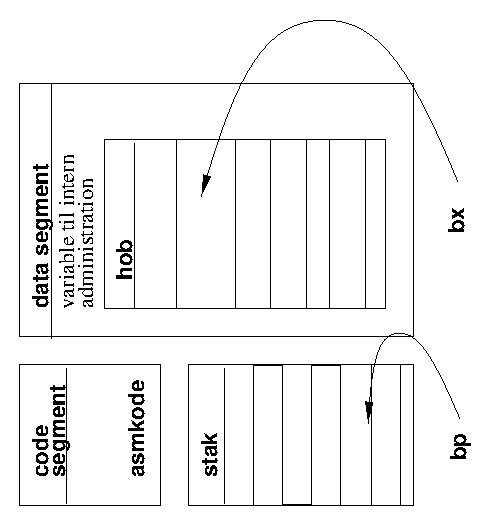
\includegraphics[angle=-90]{kodegenoversigt.ps}}}

\bigskip
\bigskip


\centerline{\fbox{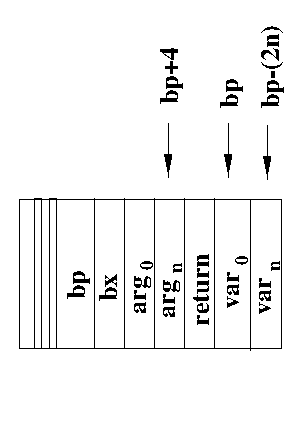
\includegraphics[angle=-90]{stak2.ps}}}

\bigskip
\bigskip


\begin{center}
\t{String s = "blabla"} \begin{tabular}{|c|}
\hline L�ngde \\ \hline \\T \\e \\g \\n \\  \\ \hline
\end{tabular}
\begin{tabular}{|c|}
\hline 6 \\ \hline b \\l \\a \\b \\l \\a \\ \hline
\end{tabular}
\end{center}



\bigskip
\bigskip

\bigskip
\bigskip

\section*{Optimering}

\begin{tabular}{|l|l|l|l|l|l|l|}
\hline
Qjava   & Qjava opt$_1$ & Qjava opt$_2$ & Qjava h�ndopt & JDK 1.3b  & C & Assembler \\
\hline
11      & 10            & 8             & 6             & 9         & 8 & 5\\
\hline
\end{tabular}

\newpage
 
\begin{verbatim}
class Prime
{
    static void main()
    {
        Prime ptr;
        ptr = new Prime();

        ptr.loop();
    }
    
    
    void loop()
    {
        int p; p = 3;
            
        while(p < 32000)
        {
            isPrime(p); p = p + 1;
        }
    }
    
            
    void isPrime(int p)
    {
        int i; i = 2;
        
        while(i < p)
        {
            if(p%i == 0){return; }
            else{i = i + 1; }
        }

        if(i == p){}
        else{}
    }
}
\end{verbatim}

\newpage

\begin{verbatim}
DOSSEG
.MODEL SMALL
.STACK 200h

.DATA

.CODE
     mov ax,@DATA
     mov ds,ax

    mov cx, 31999
again:
    mov si, 2               ; si = 2
primeTsTStart:
    cmp si, cx              ; while cx > si
    je primeTstEnd          ;
        
    mov ax, cx      
    xor dx, dx              
    div si
    cmp dx, 0               ; if cx % si == 0 then stop testing current number
    je primeTstEnd:
    inc si                  ; si++
    jmp primeTstStart
primeTstEnd:
    
    loop again              ; if cx > 0

    ; END OF SHOW
    mov ah,4ch
    int 21h

END
\end{verbatim}


\end{document}
